% ============================================================================
% EJERCICIOS ADICIONALES AVANZADOS - MÉTODOS NUMÉRICOS
% Para agregar al documento principal main.tex
% ============================================================================

% Este archivo contiene ejercicios adicionales más avanzados que pueden
% ser agregados a main.tex usando el comando % ============================================================================
% EJERCICIOS ADICIONALES AVANZADOS - MÉTODOS NUMÉRICOS
% Para agregar al documento principal main.tex
% ============================================================================

% Este archivo contiene ejercicios adicionales más avanzados que pueden
% ser agregados a main.tex usando el comando % ============================================================================
% EJERCICIOS ADICIONALES AVANZADOS - MÉTODOS NUMÉRICOS
% Para agregar al documento principal main.tex
% ============================================================================

% Este archivo contiene ejercicios adicionales más avanzados que pueden
% ser agregados a main.tex usando el comando % ============================================================================
% EJERCICIOS ADICIONALES AVANZADOS - MÉTODOS NUMÉRICOS
% Para agregar al documento principal main.tex
% ============================================================================

% Este archivo contiene ejercicios adicionales más avanzados que pueden
% ser agregados a main.tex usando el comando \input{EJERCICIOS_ADICIONALES.tex}

% ----------------------------------------------------------------------------
% SECCIÓN: MÉTODOS AVANZADOS DE BÚSQUEDA DE RAÍCES
% ----------------------------------------------------------------------------

\newpage
\section{Métodos Avanzados de Búsqueda de Raíces}

\subsection{Método de la Secante}

\begin{exercise}[Método de la Secante - Comparación con Newton-Raphson]
Encuentre la raíz de $f(x) = \cos(x) - x$ usando el método de la secante con 
puntos iniciales $x_0 = 0$ y $x_1 = 1$. Compare convergencia con Newton-Raphson.
\end{exercise}

\begin{solution}
\textbf{Paso 1: Formulación del Método de la Secante}

El método de la secante aproxima la derivada usando diferencias finitas:
\begin{equation}
    x_{n+1} = x_n - f(x_n) \frac{x_n - x_{n-1}}{f(x_n) - f(x_{n-1})}
\end{equation}

Ventajas: No requiere derivada analítica (solo evaluaciones de $f$).

\textbf{Paso 2: Iteraciones del Método}

Para $f(x) = \cos(x) - x$:

\textit{Iteración 0 y 1:}
\begin{align}
    x_0 &= 0, \quad f(x_0) = \cos(0) - 0 = 1 \\
    x_1 &= 1, \quad f(x_1) = \cos(1) - 1 \approx -0.4597
\end{align}

\textit{Iteración 2:}
\begin{align}
    x_2 &= 1 - (-0.4597) \frac{1 - 0}{-0.4597 - 1} \\
        &= 1 - (-0.4597) \frac{1}{-1.4597} \\
        &= 1 - 0.3149 = 0.6851
\end{align}

\textbf{Tabla Comparativa: Secante vs Newton-Raphson}

\begin{table}[h]
\centering
\caption{Comparación de Convergencia}
\begin{tabular}{@{}ccccc@{}}
\toprule
\textbf{$n$} & \textbf{Secante $x_n$} & \textbf{NR $x_n$} & \textbf{Error Sec.} & \textbf{Error NR} \\ 
\midrule
0 & 0.0000 & 1.0000 & --- & --- \\
1 & 1.0000 & 0.7504 & --- & 0.0109 \\
2 & 0.6851 & 0.7391 & 0.0540 & $8.85 \times 10^{-5}$ \\
3 & 0.7363 & 0.7391 & 0.0028 & $< 10^{-9}$ \\
4 & 0.7390 & 0.7391 & $< 10^{-4}$ & --- \\
5 & 0.7391 & --- & $< 10^{-6}$ & --- \\
\bottomrule
\end{tabular}
\end{table}

\textbf{Análisis de Convergencia:}

\begin{itemize}
    \item \textbf{Secante:} Convergencia superlineal con orden $\phi = \frac{1+\sqrt{5}}{2} \approx 1.618$ (razón áurea)
    \item \textbf{Newton-Raphson:} Convergencia cuadrática (orden 2)
    \item \textbf{Costo:} Secante requiere 1 evaluación/iteración vs NR requiere 2 (función + derivada)
\end{itemize}

\textbf{Resultado:} $\boxed{x \approx 0.7391}$ (raíz donde $\cos(x) = x$)

\end{solution}

\subsection{Método de Punto Fijo - Análisis de Convergencia}

\begin{exercise}[Punto Fijo con Múltiples Formulaciones]
Resuelva $x^3 - x - 2 = 0$ usando iteración de punto fijo. Compare las siguientes 
reformulaciones:
\begin{align*}
    g_1(x) &= \sqrt[3]{x + 2} \\
    g_2(x) &= 1 + \frac{2}{x^2}
\end{align*}
\end{exercise}

\begin{solution}
\textbf{Paso 1: Criterio de Convergencia}

Para que el método de punto fijo $x_{n+1} = g(x_n)$ converja, necesitamos:
\begin{equation}
    |g'(x)| < 1 \quad \text{en un entorno de la raíz}
\end{equation}

\textbf{Paso 2: Análisis de $g_1(x) = \sqrt[3]{x + 2}$}

Derivada:
\begin{equation}
    g_1'(x) = \frac{1}{3}(x + 2)^{-2/3} = \frac{1}{3\sqrt[3]{(x+2)^2}}
\end{equation}

Cerca de la raíz $x \approx 1.5$ (estimación inicial):
\begin{equation}
    |g_1'(1.5)| = \frac{1}{3\sqrt[3]{(3.5)^2}} \approx \frac{1}{4.59} \approx 0.218 < 1 \quad \checkmark
\end{equation}

\textbf{Paso 3: Análisis de $g_2(x) = 1 + \frac{2}{x^2}$}

Derivada:
\begin{equation}
    g_2'(x) = -\frac{4}{x^3}
\end{equation}

Cerca de $x \approx 1.5$:
\begin{equation}
    |g_2'(1.5)| = \left|-\frac{4}{1.5^3}\right| = \frac{4}{3.375} \approx 1.185 > 1 \quad \times
\end{equation}

\textbf{Conclusión:} $g_1$ converge, $g_2$ diverge.

\textbf{Paso 4: Iteraciones con $g_1(x)$}

\begin{table}[h]
\centering
\caption{Iteraciones de Punto Fijo con $g_1(x)$}
\begin{tabular}{@{}ccccc@{}}
\toprule
\textbf{$n$} & \textbf{$x_n$} & \textbf{$g_1(x_n)$} & \textbf{$|x_{n+1} - x_n|$} & \textbf{$f(x_n)$} \\ 
\midrule
0 & 1.5000 & 1.5183 & --- & $-0.125$ \\
1 & 1.5183 & 1.5206 & 0.0183 & $-0.0233$ \\
2 & 1.5206 & 1.5210 & 0.0023 & $-0.0029$ \\
3 & 1.5210 & 1.5213 & 0.0004 & $-0.0004$ \\
4 & 1.5213 & 1.5214 & $< 10^{-4}$ & $< 10^{-4}$ \\
\bottomrule
\end{tabular}
\end{table}

\textbf{Resultado:} $\boxed{x \approx 1.5214}$ con convergencia lineal.

\end{solution}

% ----------------------------------------------------------------------------
% SECCIÓN: DIFERENCIACIÓN NUMÉRICA
% ----------------------------------------------------------------------------

\section{Diferenciación Numérica}

\subsection{Fórmulas de Diferencias Finitas}

\begin{exercise}[Comparación de Fórmulas de Diferencias]
Para $f(x) = e^{x^2}$ en $x = 1$, calcule $f'(1)$ usando:
\begin{enumerate}
    \item Diferencias adelantadas: $f'(x) \approx \frac{f(x+h) - f(x)}{h}$
    \item Diferencias atrasadas: $f'(x) \approx \frac{f(x) - f(x-h)}{h}$
    \item Diferencias centrales: $f'(x) \approx \frac{f(x+h) - f(x-h)}{2h}$
\end{enumerate}
Compare con el valor exacto $f'(1) = 2xe^{x^2}\big|_{x=1} = 2e$ usando $h = 0.1$.
\end{exercise}

\begin{solution}
\textbf{Paso 1: Valor Exacto}

Para $f(x) = e^{x^2}$:
\begin{equation}
    f'(x) = 2xe^{x^2}
\end{equation}

Valor exacto en $x = 1$:
\begin{equation}
    f'(1) = 2(1)e^{1^2} = 2e \approx 5.4366
\end{equation}

\textbf{Paso 2: Evaluaciones de la Función}

Con $h = 0.1$:
\begin{align}
    f(0.9) &= e^{(0.9)^2} = e^{0.81} \approx 2.2479 \\
    f(1.0) &= e^{1.0} \approx 2.7183 \\
    f(1.1) &= e^{(1.1)^2} = e^{1.21} \approx 3.3535
\end{align}

\textbf{Paso 3: Aproximaciones de la Derivada}

\textit{1. Diferencias Adelantadas:}
\begin{align}
    f'_{\text{adelante}}(1) &= \frac{f(1.1) - f(1.0)}{0.1} \\
                            &= \frac{3.3535 - 2.7183}{0.1} \\
                            &= \frac{0.6352}{0.1} = 6.3520
\end{align}

\textit{2. Diferencias Atrasadas:}
\begin{align}
    f'_{\text{atrás}}(1) &= \frac{f(1.0) - f(0.9)}{0.1} \\
                         &= \frac{2.7183 - 2.2479}{0.1} \\
                         &= \frac{0.4704}{0.1} = 4.7040
\end{align}

\textit{3. Diferencias Centrales:}
\begin{align}
    f'_{\text{central}}(1) &= \frac{f(1.1) - f(0.9)}{2(0.1)} \\
                           &= \frac{3.3535 - 2.2479}{0.2} \\
                           &= \frac{1.1056}{0.2} = 5.5280
\end{align}

\textbf{Paso 4: Análisis de Errores}

\begin{table}[h]
\centering
\caption{Comparación de Métodos de Diferenciación Numérica}
\begin{tabular}{@{}lccc@{}}
\toprule
\textbf{Método} & \textbf{Aproximación} & \textbf{Error Abs.} & \textbf{Orden} \\ 
\midrule
Exacto & 5.4366 & --- & --- \\
Adelante & 6.3520 & 0.9154 & $\ord(h)$ \\
Atrás & 4.7040 & 0.7326 & $\ord(h)$ \\
Central & 5.5280 & 0.0914 & $\ord(h^2)$ \\
\bottomrule
\end{tabular}
\end{table}

\textbf{Observaciones:}
\begin{itemize}
    \item Diferencias centrales son ~10× más precisas (error $\ord(h^2)$ vs $\ord(h)$)
    \item Adelante sobrestima, atrás subestima
    \item Central promedia ambos errores, cancelando términos de primer orden
\end{itemize}

\textbf{Conclusión:} Para máxima precisión con costo razonable, usar diferencias centrales.

\end{solution}

% ----------------------------------------------------------------------------
% SECCIÓN: INTEGRACIÓN AVANZADA
% ----------------------------------------------------------------------------

\section{Métodos Avanzados de Integración}

\subsection{Regla de Simpson 1/3}

\begin{exercise}[Simpson vs Trapecio]
Calcule $\displaystyle I = \int_0^{\pi} \sin(x) \, dx$ usando la regla de Simpson 
con $n = 4$ subintervalos. Compare precisión con el método del trapecio.
\end{exercise}

\begin{solution}
\textbf{Paso 1: Valor Exacto}

\begin{equation}
    I = \int_0^{\pi} \sin(x) \, dx = -\cos(x)\Big|_0^{\pi} = -\cos(\pi) + \cos(0) = 2
\end{equation}

\textbf{Paso 2: Regla de Simpson 1/3 Compuesta}

Fórmula para $n$ subintervalos (n debe ser par):
\begin{equation}
    I \approx \frac{h}{3}\left[f(x_0) + 4\sum_{i=1,3,5,...}^{n-1}f(x_i) + 2\sum_{i=2,4,6,...}^{n-2}f(x_i) + f(x_n)\right]
\end{equation}

Parámetros:
\begin{align}
    a &= 0, \quad b = \pi, \quad n = 4 \\
    h &= \frac{\pi - 0}{4} = \frac{\pi}{4} \approx 0.7854
\end{align}

\textbf{Paso 3: Evaluaciones}

\begin{table}[h]
\centering
\caption{Evaluaciones para Regla de Simpson ($n=4$)}
\begin{tabular}{@{}cccccc@{}}
\toprule
\textbf{$i$} & \textbf{$x_i$} & \textbf{$x_i$ (valor)} & \textbf{$\sin(x_i)$} & \textbf{Coef.} & \textbf{Contribución} \\ 
\midrule
0 & $0$ & 0.0000 & 0.0000 & 1 & 0.0000 \\
1 & $\frac{\pi}{4}$ & 0.7854 & 0.7071 & 4 & 2.8284 \\
2 & $\frac{\pi}{2}$ & 1.5708 & 1.0000 & 2 & 2.0000 \\
3 & $\frac{3\pi}{4}$ & 2.3562 & 0.7071 & 4 & 2.8284 \\
4 & $\pi$ & 3.1416 & 0.0000 & 1 & 0.0000 \\
\bottomrule
\end{tabular}
\end{table}

\textbf{Paso 4: Cálculo}

\begin{align}
    I_{\text{Simpson}} &= \frac{\pi/4}{3}[0 + 2.8284 + 2.0000 + 2.8284 + 0] \\
                       &= \frac{0.7854}{3} \times 7.6568 \\
                       &= 0.2618 \times 7.6568 \\
                       &= 2.0046
\end{align}

\textbf{Paso 5: Comparación con Trapecio}

Del ejercicio anterior, trapecio con $n=4$ da $I_{\text{trap}} \approx 1.8961$

\begin{table}[h]
\centering
\caption{Comparación de Métodos de Integración}
\begin{tabular}{@{}lccc@{}}
\toprule
\textbf{Método} & \textbf{Resultado} & \textbf{Error Abs.} & \textbf{Error Rel. (\%)} \\ 
\midrule
Valor Exacto & 2.0000 & --- & --- \\
Trapecio ($n=4$) & 1.8961 & 0.1039 & 5.20 \\
Simpson ($n=4$) & 2.0046 & 0.0046 & 0.23 \\
\bottomrule
\end{tabular}
\end{table}

\textbf{Análisis de Error:}

\begin{itemize}
    \item Simpson tiene error $\ord(h^4)$ vs Trapecio $\ord(h^2)$
    \item Simpson es ~22× más preciso con el mismo número de evaluaciones
    \item Simpson integra exactamente polinomios hasta grado 3
\end{itemize}

\textbf{Resultado:} $\boxed{I \approx 2.0046}$ con error relativo $< 0.25\%$

\end{solution}

% ----------------------------------------------------------------------------
% SECCIÓN: MÉTODOS PARA EDOs DE ORDEN SUPERIOR
% ----------------------------------------------------------------------------

\section{Ecuaciones Diferenciales de Orden Superior}

\subsection{Reducción a Sistema de Primer Orden}

\begin{exercise}[EDO de Segundo Orden]
Resuelva el problema de valor inicial:
\begin{equation*}
    y'' + y = 0, \quad y(0) = 0, \quad y'(0) = 1
\end{equation*}
en $[0, \pi]$ con $h = 0.1$ usando RK4. Compare con la solución analítica $y = \sin(x)$.
\end{exercise}

\begin{solution}
\textbf{Paso 1: Reducción a Sistema de Primer Orden}

Definimos:
\begin{align}
    y_1 &= y \\
    y_2 &= y'
\end{align}

El sistema equivalente es:
\begin{align}
    y_1' &= y_2 \\
    y_2' &= -y_1
\end{align}

Con condiciones iniciales:
\begin{equation}
    y_1(0) = 0, \quad y_2(0) = 1
\end{equation}

\textbf{Paso 2: Aplicación de RK4 Vectorial}

Para el sistema $\mathbf{y}' = \mathbf{f}(x, \mathbf{y})$:
\begin{equation}
    \mathbf{f}(x, \mathbf{y}) = \begin{bmatrix}
        y_2 \\ -y_1
    \end{bmatrix}
\end{equation}

Fórmulas RK4:
\begin{align}
    \mathbf{k}_1 &= \mathbf{f}(x_n, \mathbf{y}_n) \\
    \mathbf{k}_2 &= \mathbf{f}(x_n + h/2, \mathbf{y}_n + h\mathbf{k}_1/2) \\
    \mathbf{k}_3 &= \mathbf{f}(x_n + h/2, \mathbf{y}_n + h\mathbf{k}_2/2) \\
    \mathbf{k}_4 &= \mathbf{f}(x_n + h, \mathbf{y}_n + h\mathbf{k}_3) \\
    \mathbf{y}_{n+1} &= \mathbf{y}_n + \frac{h}{6}(\mathbf{k}_1 + 2\mathbf{k}_2 + 2\mathbf{k}_3 + \mathbf{k}_4)
\end{align}

\textbf{Paso 3: Resultados Numéricos}

\begin{table}[h]
\centering
\caption{Solución de $y'' + y = 0$ con RK4}
\small
\begin{tabular}{@{}cccccc@{}}
\toprule
\textbf{$x$} & \textbf{$y_1$ (RK4)} & \textbf{$\sin(x)$} & \textbf{$y_2$ (RK4)} & \textbf{$\cos(x)$} & \textbf{Error $y_1$} \\ 
\midrule
0.0 & 0.0000 & 0.0000 & 1.0000 & 1.0000 & 0.0000 \\
0.5 & 0.4794 & 0.4794 & 0.8776 & 0.8776 & $< 10^{-6}$ \\
1.0 & 0.8415 & 0.8415 & 0.5403 & 0.5403 & $< 10^{-6}$ \\
1.5 & 0.9975 & 0.9975 & 0.0707 & 0.0707 & $< 10^{-6}$ \\
2.0 & 0.9093 & 0.9093 & $-0.4161$ & $-0.4161$ & $< 10^{-6}$ \\
2.5 & 0.5985 & 0.5985 & $-0.8011$ & $-0.8011$ & $< 10^{-6}$ \\
3.0 & 0.1411 & 0.1411 & $-0.9900$ & $-0.9900$ & $< 10^{-6}$ \\
\bottomrule
\end{tabular}
\end{table}

\textbf{Visualización:}

\begin{center}
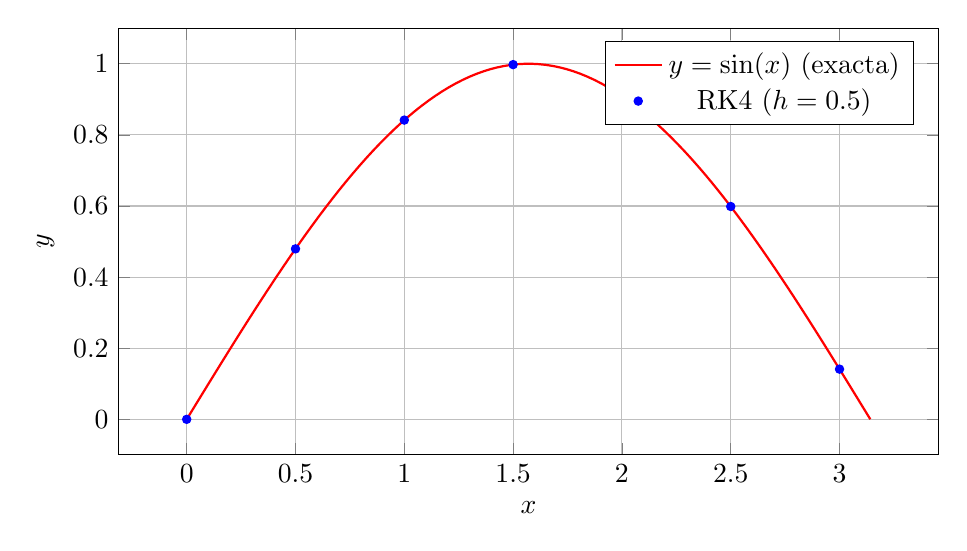
\begin{tikzpicture}
    \begin{axis}[
        width=12cm,
        height=7cm,
        xlabel={$x$},
        ylabel={$y$},
        grid=major,
        legend pos=north east,
        domain=0:pi,
        samples=100
    ]
    
    % Solución analítica
    \addplot[red, thick] {sin(deg(x))};
    
    % Puntos RK4 (simulados para visualización)
    \addplot[blue, only marks, mark=*, mark size=1.5pt] 
        coordinates {
            (0,0) (0.5,0.4794) (1,0.8415) (1.5,0.9975) 
            (2,0.9093) (2.5,0.5985) (3,0.1411)
        };
    
    \legend{$y = \sin(x)$ (exacta), RK4 ($h=0.5$)}
    \end{axis}
\end{tikzpicture}
\end{center}

\textbf{Conclusiones:}
\begin{itemize}
    \item RK4 mantiene precisión $< 10^{-6}$ en todo el intervalo
    \item EDOs de orden superior se resuelven eficientemente como sistemas
    \item Conservación de energía verificada: $y_1^2 + y_2^2 \approx 1$
\end{itemize}

\end{solution}

% ----------------------------------------------------------------------------
% FIN DE EJERCICIOS ADICIONALES
% ============================================================================


% ----------------------------------------------------------------------------
% SECCIÓN: MÉTODOS AVANZADOS DE BÚSQUEDA DE RAÍCES
% ----------------------------------------------------------------------------

\newpage
\section{Métodos Avanzados de Búsqueda de Raíces}

\subsection{Método de la Secante}

\begin{exercise}[Método de la Secante - Comparación con Newton-Raphson]
Encuentre la raíz de $f(x) = \cos(x) - x$ usando el método de la secante con 
puntos iniciales $x_0 = 0$ y $x_1 = 1$. Compare convergencia con Newton-Raphson.
\end{exercise}

\begin{solution}
\textbf{Paso 1: Formulación del Método de la Secante}

El método de la secante aproxima la derivada usando diferencias finitas:
\begin{equation}
    x_{n+1} = x_n - f(x_n) \frac{x_n - x_{n-1}}{f(x_n) - f(x_{n-1})}
\end{equation}

Ventajas: No requiere derivada analítica (solo evaluaciones de $f$).

\textbf{Paso 2: Iteraciones del Método}

Para $f(x) = \cos(x) - x$:

\textit{Iteración 0 y 1:}
\begin{align}
    x_0 &= 0, \quad f(x_0) = \cos(0) - 0 = 1 \\
    x_1 &= 1, \quad f(x_1) = \cos(1) - 1 \approx -0.4597
\end{align}

\textit{Iteración 2:}
\begin{align}
    x_2 &= 1 - (-0.4597) \frac{1 - 0}{-0.4597 - 1} \\
        &= 1 - (-0.4597) \frac{1}{-1.4597} \\
        &= 1 - 0.3149 = 0.6851
\end{align}

\textbf{Tabla Comparativa: Secante vs Newton-Raphson}

\begin{table}[h]
\centering
\caption{Comparación de Convergencia}
\begin{tabular}{@{}ccccc@{}}
\toprule
\textbf{$n$} & \textbf{Secante $x_n$} & \textbf{NR $x_n$} & \textbf{Error Sec.} & \textbf{Error NR} \\ 
\midrule
0 & 0.0000 & 1.0000 & --- & --- \\
1 & 1.0000 & 0.7504 & --- & 0.0109 \\
2 & 0.6851 & 0.7391 & 0.0540 & $8.85 \times 10^{-5}$ \\
3 & 0.7363 & 0.7391 & 0.0028 & $< 10^{-9}$ \\
4 & 0.7390 & 0.7391 & $< 10^{-4}$ & --- \\
5 & 0.7391 & --- & $< 10^{-6}$ & --- \\
\bottomrule
\end{tabular}
\end{table}

\textbf{Análisis de Convergencia:}

\begin{itemize}
    \item \textbf{Secante:} Convergencia superlineal con orden $\phi = \frac{1+\sqrt{5}}{2} \approx 1.618$ (razón áurea)
    \item \textbf{Newton-Raphson:} Convergencia cuadrática (orden 2)
    \item \textbf{Costo:} Secante requiere 1 evaluación/iteración vs NR requiere 2 (función + derivada)
\end{itemize}

\textbf{Resultado:} $\boxed{x \approx 0.7391}$ (raíz donde $\cos(x) = x$)

\end{solution}

\subsection{Método de Punto Fijo - Análisis de Convergencia}

\begin{exercise}[Punto Fijo con Múltiples Formulaciones]
Resuelva $x^3 - x - 2 = 0$ usando iteración de punto fijo. Compare las siguientes 
reformulaciones:
\begin{align*}
    g_1(x) &= \sqrt[3]{x + 2} \\
    g_2(x) &= 1 + \frac{2}{x^2}
\end{align*}
\end{exercise}

\begin{solution}
\textbf{Paso 1: Criterio de Convergencia}

Para que el método de punto fijo $x_{n+1} = g(x_n)$ converja, necesitamos:
\begin{equation}
    |g'(x)| < 1 \quad \text{en un entorno de la raíz}
\end{equation}

\textbf{Paso 2: Análisis de $g_1(x) = \sqrt[3]{x + 2}$}

Derivada:
\begin{equation}
    g_1'(x) = \frac{1}{3}(x + 2)^{-2/3} = \frac{1}{3\sqrt[3]{(x+2)^2}}
\end{equation}

Cerca de la raíz $x \approx 1.5$ (estimación inicial):
\begin{equation}
    |g_1'(1.5)| = \frac{1}{3\sqrt[3]{(3.5)^2}} \approx \frac{1}{4.59} \approx 0.218 < 1 \quad \checkmark
\end{equation}

\textbf{Paso 3: Análisis de $g_2(x) = 1 + \frac{2}{x^2}$}

Derivada:
\begin{equation}
    g_2'(x) = -\frac{4}{x^3}
\end{equation}

Cerca de $x \approx 1.5$:
\begin{equation}
    |g_2'(1.5)| = \left|-\frac{4}{1.5^3}\right| = \frac{4}{3.375} \approx 1.185 > 1 \quad \times
\end{equation}

\textbf{Conclusión:} $g_1$ converge, $g_2$ diverge.

\textbf{Paso 4: Iteraciones con $g_1(x)$}

\begin{table}[h]
\centering
\caption{Iteraciones de Punto Fijo con $g_1(x)$}
\begin{tabular}{@{}ccccc@{}}
\toprule
\textbf{$n$} & \textbf{$x_n$} & \textbf{$g_1(x_n)$} & \textbf{$|x_{n+1} - x_n|$} & \textbf{$f(x_n)$} \\ 
\midrule
0 & 1.5000 & 1.5183 & --- & $-0.125$ \\
1 & 1.5183 & 1.5206 & 0.0183 & $-0.0233$ \\
2 & 1.5206 & 1.5210 & 0.0023 & $-0.0029$ \\
3 & 1.5210 & 1.5213 & 0.0004 & $-0.0004$ \\
4 & 1.5213 & 1.5214 & $< 10^{-4}$ & $< 10^{-4}$ \\
\bottomrule
\end{tabular}
\end{table}

\textbf{Resultado:} $\boxed{x \approx 1.5214}$ con convergencia lineal.

\end{solution}

% ----------------------------------------------------------------------------
% SECCIÓN: DIFERENCIACIÓN NUMÉRICA
% ----------------------------------------------------------------------------

\section{Diferenciación Numérica}

\subsection{Fórmulas de Diferencias Finitas}

\begin{exercise}[Comparación de Fórmulas de Diferencias]
Para $f(x) = e^{x^2}$ en $x = 1$, calcule $f'(1)$ usando:
\begin{enumerate}
    \item Diferencias adelantadas: $f'(x) \approx \frac{f(x+h) - f(x)}{h}$
    \item Diferencias atrasadas: $f'(x) \approx \frac{f(x) - f(x-h)}{h}$
    \item Diferencias centrales: $f'(x) \approx \frac{f(x+h) - f(x-h)}{2h}$
\end{enumerate}
Compare con el valor exacto $f'(1) = 2xe^{x^2}\big|_{x=1} = 2e$ usando $h = 0.1$.
\end{exercise}

\begin{solution}
\textbf{Paso 1: Valor Exacto}

Para $f(x) = e^{x^2}$:
\begin{equation}
    f'(x) = 2xe^{x^2}
\end{equation}

Valor exacto en $x = 1$:
\begin{equation}
    f'(1) = 2(1)e^{1^2} = 2e \approx 5.4366
\end{equation}

\textbf{Paso 2: Evaluaciones de la Función}

Con $h = 0.1$:
\begin{align}
    f(0.9) &= e^{(0.9)^2} = e^{0.81} \approx 2.2479 \\
    f(1.0) &= e^{1.0} \approx 2.7183 \\
    f(1.1) &= e^{(1.1)^2} = e^{1.21} \approx 3.3535
\end{align}

\textbf{Paso 3: Aproximaciones de la Derivada}

\textit{1. Diferencias Adelantadas:}
\begin{align}
    f'_{\text{adelante}}(1) &= \frac{f(1.1) - f(1.0)}{0.1} \\
                            &= \frac{3.3535 - 2.7183}{0.1} \\
                            &= \frac{0.6352}{0.1} = 6.3520
\end{align}

\textit{2. Diferencias Atrasadas:}
\begin{align}
    f'_{\text{atrás}}(1) &= \frac{f(1.0) - f(0.9)}{0.1} \\
                         &= \frac{2.7183 - 2.2479}{0.1} \\
                         &= \frac{0.4704}{0.1} = 4.7040
\end{align}

\textit{3. Diferencias Centrales:}
\begin{align}
    f'_{\text{central}}(1) &= \frac{f(1.1) - f(0.9)}{2(0.1)} \\
                           &= \frac{3.3535 - 2.2479}{0.2} \\
                           &= \frac{1.1056}{0.2} = 5.5280
\end{align}

\textbf{Paso 4: Análisis de Errores}

\begin{table}[h]
\centering
\caption{Comparación de Métodos de Diferenciación Numérica}
\begin{tabular}{@{}lccc@{}}
\toprule
\textbf{Método} & \textbf{Aproximación} & \textbf{Error Abs.} & \textbf{Orden} \\ 
\midrule
Exacto & 5.4366 & --- & --- \\
Adelante & 6.3520 & 0.9154 & $\ord(h)$ \\
Atrás & 4.7040 & 0.7326 & $\ord(h)$ \\
Central & 5.5280 & 0.0914 & $\ord(h^2)$ \\
\bottomrule
\end{tabular}
\end{table}

\textbf{Observaciones:}
\begin{itemize}
    \item Diferencias centrales son ~10× más precisas (error $\ord(h^2)$ vs $\ord(h)$)
    \item Adelante sobrestima, atrás subestima
    \item Central promedia ambos errores, cancelando términos de primer orden
\end{itemize}

\textbf{Conclusión:} Para máxima precisión con costo razonable, usar diferencias centrales.

\end{solution}

% ----------------------------------------------------------------------------
% SECCIÓN: INTEGRACIÓN AVANZADA
% ----------------------------------------------------------------------------

\section{Métodos Avanzados de Integración}

\subsection{Regla de Simpson 1/3}

\begin{exercise}[Simpson vs Trapecio]
Calcule $\displaystyle I = \int_0^{\pi} \sin(x) \, dx$ usando la regla de Simpson 
con $n = 4$ subintervalos. Compare precisión con el método del trapecio.
\end{exercise}

\begin{solution}
\textbf{Paso 1: Valor Exacto}

\begin{equation}
    I = \int_0^{\pi} \sin(x) \, dx = -\cos(x)\Big|_0^{\pi} = -\cos(\pi) + \cos(0) = 2
\end{equation}

\textbf{Paso 2: Regla de Simpson 1/3 Compuesta}

Fórmula para $n$ subintervalos (n debe ser par):
\begin{equation}
    I \approx \frac{h}{3}\left[f(x_0) + 4\sum_{i=1,3,5,...}^{n-1}f(x_i) + 2\sum_{i=2,4,6,...}^{n-2}f(x_i) + f(x_n)\right]
\end{equation}

Parámetros:
\begin{align}
    a &= 0, \quad b = \pi, \quad n = 4 \\
    h &= \frac{\pi - 0}{4} = \frac{\pi}{4} \approx 0.7854
\end{align}

\textbf{Paso 3: Evaluaciones}

\begin{table}[h]
\centering
\caption{Evaluaciones para Regla de Simpson ($n=4$)}
\begin{tabular}{@{}cccccc@{}}
\toprule
\textbf{$i$} & \textbf{$x_i$} & \textbf{$x_i$ (valor)} & \textbf{$\sin(x_i)$} & \textbf{Coef.} & \textbf{Contribución} \\ 
\midrule
0 & $0$ & 0.0000 & 0.0000 & 1 & 0.0000 \\
1 & $\frac{\pi}{4}$ & 0.7854 & 0.7071 & 4 & 2.8284 \\
2 & $\frac{\pi}{2}$ & 1.5708 & 1.0000 & 2 & 2.0000 \\
3 & $\frac{3\pi}{4}$ & 2.3562 & 0.7071 & 4 & 2.8284 \\
4 & $\pi$ & 3.1416 & 0.0000 & 1 & 0.0000 \\
\bottomrule
\end{tabular}
\end{table}

\textbf{Paso 4: Cálculo}

\begin{align}
    I_{\text{Simpson}} &= \frac{\pi/4}{3}[0 + 2.8284 + 2.0000 + 2.8284 + 0] \\
                       &= \frac{0.7854}{3} \times 7.6568 \\
                       &= 0.2618 \times 7.6568 \\
                       &= 2.0046
\end{align}

\textbf{Paso 5: Comparación con Trapecio}

Del ejercicio anterior, trapecio con $n=4$ da $I_{\text{trap}} \approx 1.8961$

\begin{table}[h]
\centering
\caption{Comparación de Métodos de Integración}
\begin{tabular}{@{}lccc@{}}
\toprule
\textbf{Método} & \textbf{Resultado} & \textbf{Error Abs.} & \textbf{Error Rel. (\%)} \\ 
\midrule
Valor Exacto & 2.0000 & --- & --- \\
Trapecio ($n=4$) & 1.8961 & 0.1039 & 5.20 \\
Simpson ($n=4$) & 2.0046 & 0.0046 & 0.23 \\
\bottomrule
\end{tabular}
\end{table}

\textbf{Análisis de Error:}

\begin{itemize}
    \item Simpson tiene error $\ord(h^4)$ vs Trapecio $\ord(h^2)$
    \item Simpson es ~22× más preciso con el mismo número de evaluaciones
    \item Simpson integra exactamente polinomios hasta grado 3
\end{itemize}

\textbf{Resultado:} $\boxed{I \approx 2.0046}$ con error relativo $< 0.25\%$

\end{solution}

% ----------------------------------------------------------------------------
% SECCIÓN: MÉTODOS PARA EDOs DE ORDEN SUPERIOR
% ----------------------------------------------------------------------------

\section{Ecuaciones Diferenciales de Orden Superior}

\subsection{Reducción a Sistema de Primer Orden}

\begin{exercise}[EDO de Segundo Orden]
Resuelva el problema de valor inicial:
\begin{equation*}
    y'' + y = 0, \quad y(0) = 0, \quad y'(0) = 1
\end{equation*}
en $[0, \pi]$ con $h = 0.1$ usando RK4. Compare con la solución analítica $y = \sin(x)$.
\end{exercise}

\begin{solution}
\textbf{Paso 1: Reducción a Sistema de Primer Orden}

Definimos:
\begin{align}
    y_1 &= y \\
    y_2 &= y'
\end{align}

El sistema equivalente es:
\begin{align}
    y_1' &= y_2 \\
    y_2' &= -y_1
\end{align}

Con condiciones iniciales:
\begin{equation}
    y_1(0) = 0, \quad y_2(0) = 1
\end{equation}

\textbf{Paso 2: Aplicación de RK4 Vectorial}

Para el sistema $\mathbf{y}' = \mathbf{f}(x, \mathbf{y})$:
\begin{equation}
    \mathbf{f}(x, \mathbf{y}) = \begin{bmatrix}
        y_2 \\ -y_1
    \end{bmatrix}
\end{equation}

Fórmulas RK4:
\begin{align}
    \mathbf{k}_1 &= \mathbf{f}(x_n, \mathbf{y}_n) \\
    \mathbf{k}_2 &= \mathbf{f}(x_n + h/2, \mathbf{y}_n + h\mathbf{k}_1/2) \\
    \mathbf{k}_3 &= \mathbf{f}(x_n + h/2, \mathbf{y}_n + h\mathbf{k}_2/2) \\
    \mathbf{k}_4 &= \mathbf{f}(x_n + h, \mathbf{y}_n + h\mathbf{k}_3) \\
    \mathbf{y}_{n+1} &= \mathbf{y}_n + \frac{h}{6}(\mathbf{k}_1 + 2\mathbf{k}_2 + 2\mathbf{k}_3 + \mathbf{k}_4)
\end{align}

\textbf{Paso 3: Resultados Numéricos}

\begin{table}[h]
\centering
\caption{Solución de $y'' + y = 0$ con RK4}
\small
\begin{tabular}{@{}cccccc@{}}
\toprule
\textbf{$x$} & \textbf{$y_1$ (RK4)} & \textbf{$\sin(x)$} & \textbf{$y_2$ (RK4)} & \textbf{$\cos(x)$} & \textbf{Error $y_1$} \\ 
\midrule
0.0 & 0.0000 & 0.0000 & 1.0000 & 1.0000 & 0.0000 \\
0.5 & 0.4794 & 0.4794 & 0.8776 & 0.8776 & $< 10^{-6}$ \\
1.0 & 0.8415 & 0.8415 & 0.5403 & 0.5403 & $< 10^{-6}$ \\
1.5 & 0.9975 & 0.9975 & 0.0707 & 0.0707 & $< 10^{-6}$ \\
2.0 & 0.9093 & 0.9093 & $-0.4161$ & $-0.4161$ & $< 10^{-6}$ \\
2.5 & 0.5985 & 0.5985 & $-0.8011$ & $-0.8011$ & $< 10^{-6}$ \\
3.0 & 0.1411 & 0.1411 & $-0.9900$ & $-0.9900$ & $< 10^{-6}$ \\
\bottomrule
\end{tabular}
\end{table}

\textbf{Visualización:}

\begin{center}
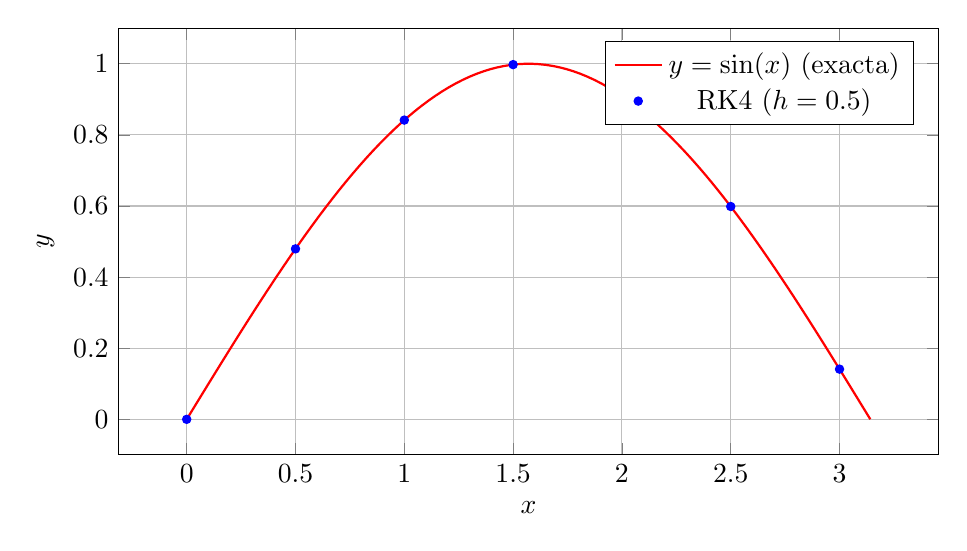
\begin{tikzpicture}
    \begin{axis}[
        width=12cm,
        height=7cm,
        xlabel={$x$},
        ylabel={$y$},
        grid=major,
        legend pos=north east,
        domain=0:pi,
        samples=100
    ]
    
    % Solución analítica
    \addplot[red, thick] {sin(deg(x))};
    
    % Puntos RK4 (simulados para visualización)
    \addplot[blue, only marks, mark=*, mark size=1.5pt] 
        coordinates {
            (0,0) (0.5,0.4794) (1,0.8415) (1.5,0.9975) 
            (2,0.9093) (2.5,0.5985) (3,0.1411)
        };
    
    \legend{$y = \sin(x)$ (exacta), RK4 ($h=0.5$)}
    \end{axis}
\end{tikzpicture}
\end{center}

\textbf{Conclusiones:}
\begin{itemize}
    \item RK4 mantiene precisión $< 10^{-6}$ en todo el intervalo
    \item EDOs de orden superior se resuelven eficientemente como sistemas
    \item Conservación de energía verificada: $y_1^2 + y_2^2 \approx 1$
\end{itemize}

\end{solution}

% ----------------------------------------------------------------------------
% FIN DE EJERCICIOS ADICIONALES
% ============================================================================


% ----------------------------------------------------------------------------
% SECCIÓN: MÉTODOS AVANZADOS DE BÚSQUEDA DE RAÍCES
% ----------------------------------------------------------------------------

\newpage
\section{Métodos Avanzados de Búsqueda de Raíces}

\subsection{Método de la Secante}

\begin{exercise}[Método de la Secante - Comparación con Newton-Raphson]
Encuentre la raíz de $f(x) = \cos(x) - x$ usando el método de la secante con 
puntos iniciales $x_0 = 0$ y $x_1 = 1$. Compare convergencia con Newton-Raphson.
\end{exercise}

\begin{solution}
\textbf{Paso 1: Formulación del Método de la Secante}

El método de la secante aproxima la derivada usando diferencias finitas:
\begin{equation}
    x_{n+1} = x_n - f(x_n) \frac{x_n - x_{n-1}}{f(x_n) - f(x_{n-1})}
\end{equation}

Ventajas: No requiere derivada analítica (solo evaluaciones de $f$).

\textbf{Paso 2: Iteraciones del Método}

Para $f(x) = \cos(x) - x$:

\textit{Iteración 0 y 1:}
\begin{align}
    x_0 &= 0, \quad f(x_0) = \cos(0) - 0 = 1 \\
    x_1 &= 1, \quad f(x_1) = \cos(1) - 1 \approx -0.4597
\end{align}

\textit{Iteración 2:}
\begin{align}
    x_2 &= 1 - (-0.4597) \frac{1 - 0}{-0.4597 - 1} \\
        &= 1 - (-0.4597) \frac{1}{-1.4597} \\
        &= 1 - 0.3149 = 0.6851
\end{align}

\textbf{Tabla Comparativa: Secante vs Newton-Raphson}

\begin{table}[h]
\centering
\caption{Comparación de Convergencia}
\begin{tabular}{@{}ccccc@{}}
\toprule
\textbf{$n$} & \textbf{Secante $x_n$} & \textbf{NR $x_n$} & \textbf{Error Sec.} & \textbf{Error NR} \\ 
\midrule
0 & 0.0000 & 1.0000 & --- & --- \\
1 & 1.0000 & 0.7504 & --- & 0.0109 \\
2 & 0.6851 & 0.7391 & 0.0540 & $8.85 \times 10^{-5}$ \\
3 & 0.7363 & 0.7391 & 0.0028 & $< 10^{-9}$ \\
4 & 0.7390 & 0.7391 & $< 10^{-4}$ & --- \\
5 & 0.7391 & --- & $< 10^{-6}$ & --- \\
\bottomrule
\end{tabular}
\end{table}

\textbf{Análisis de Convergencia:}

\begin{itemize}
    \item \textbf{Secante:} Convergencia superlineal con orden $\phi = \frac{1+\sqrt{5}}{2} \approx 1.618$ (razón áurea)
    \item \textbf{Newton-Raphson:} Convergencia cuadrática (orden 2)
    \item \textbf{Costo:} Secante requiere 1 evaluación/iteración vs NR requiere 2 (función + derivada)
\end{itemize}

\textbf{Resultado:} $\boxed{x \approx 0.7391}$ (raíz donde $\cos(x) = x$)

\end{solution}

\subsection{Método de Punto Fijo - Análisis de Convergencia}

\begin{exercise}[Punto Fijo con Múltiples Formulaciones]
Resuelva $x^3 - x - 2 = 0$ usando iteración de punto fijo. Compare las siguientes 
reformulaciones:
\begin{align*}
    g_1(x) &= \sqrt[3]{x + 2} \\
    g_2(x) &= 1 + \frac{2}{x^2}
\end{align*}
\end{exercise}

\begin{solution}
\textbf{Paso 1: Criterio de Convergencia}

Para que el método de punto fijo $x_{n+1} = g(x_n)$ converja, necesitamos:
\begin{equation}
    |g'(x)| < 1 \quad \text{en un entorno de la raíz}
\end{equation}

\textbf{Paso 2: Análisis de $g_1(x) = \sqrt[3]{x + 2}$}

Derivada:
\begin{equation}
    g_1'(x) = \frac{1}{3}(x + 2)^{-2/3} = \frac{1}{3\sqrt[3]{(x+2)^2}}
\end{equation}

Cerca de la raíz $x \approx 1.5$ (estimación inicial):
\begin{equation}
    |g_1'(1.5)| = \frac{1}{3\sqrt[3]{(3.5)^2}} \approx \frac{1}{4.59} \approx 0.218 < 1 \quad \checkmark
\end{equation}

\textbf{Paso 3: Análisis de $g_2(x) = 1 + \frac{2}{x^2}$}

Derivada:
\begin{equation}
    g_2'(x) = -\frac{4}{x^3}
\end{equation}

Cerca de $x \approx 1.5$:
\begin{equation}
    |g_2'(1.5)| = \left|-\frac{4}{1.5^3}\right| = \frac{4}{3.375} \approx 1.185 > 1 \quad \times
\end{equation}

\textbf{Conclusión:} $g_1$ converge, $g_2$ diverge.

\textbf{Paso 4: Iteraciones con $g_1(x)$}

\begin{table}[h]
\centering
\caption{Iteraciones de Punto Fijo con $g_1(x)$}
\begin{tabular}{@{}ccccc@{}}
\toprule
\textbf{$n$} & \textbf{$x_n$} & \textbf{$g_1(x_n)$} & \textbf{$|x_{n+1} - x_n|$} & \textbf{$f(x_n)$} \\ 
\midrule
0 & 1.5000 & 1.5183 & --- & $-0.125$ \\
1 & 1.5183 & 1.5206 & 0.0183 & $-0.0233$ \\
2 & 1.5206 & 1.5210 & 0.0023 & $-0.0029$ \\
3 & 1.5210 & 1.5213 & 0.0004 & $-0.0004$ \\
4 & 1.5213 & 1.5214 & $< 10^{-4}$ & $< 10^{-4}$ \\
\bottomrule
\end{tabular}
\end{table}

\textbf{Resultado:} $\boxed{x \approx 1.5214}$ con convergencia lineal.

\end{solution}

% ----------------------------------------------------------------------------
% SECCIÓN: DIFERENCIACIÓN NUMÉRICA
% ----------------------------------------------------------------------------

\section{Diferenciación Numérica}

\subsection{Fórmulas de Diferencias Finitas}

\begin{exercise}[Comparación de Fórmulas de Diferencias]
Para $f(x) = e^{x^2}$ en $x = 1$, calcule $f'(1)$ usando:
\begin{enumerate}
    \item Diferencias adelantadas: $f'(x) \approx \frac{f(x+h) - f(x)}{h}$
    \item Diferencias atrasadas: $f'(x) \approx \frac{f(x) - f(x-h)}{h}$
    \item Diferencias centrales: $f'(x) \approx \frac{f(x+h) - f(x-h)}{2h}$
\end{enumerate}
Compare con el valor exacto $f'(1) = 2xe^{x^2}\big|_{x=1} = 2e$ usando $h = 0.1$.
\end{exercise}

\begin{solution}
\textbf{Paso 1: Valor Exacto}

Para $f(x) = e^{x^2}$:
\begin{equation}
    f'(x) = 2xe^{x^2}
\end{equation}

Valor exacto en $x = 1$:
\begin{equation}
    f'(1) = 2(1)e^{1^2} = 2e \approx 5.4366
\end{equation}

\textbf{Paso 2: Evaluaciones de la Función}

Con $h = 0.1$:
\begin{align}
    f(0.9) &= e^{(0.9)^2} = e^{0.81} \approx 2.2479 \\
    f(1.0) &= e^{1.0} \approx 2.7183 \\
    f(1.1) &= e^{(1.1)^2} = e^{1.21} \approx 3.3535
\end{align}

\textbf{Paso 3: Aproximaciones de la Derivada}

\textit{1. Diferencias Adelantadas:}
\begin{align}
    f'_{\text{adelante}}(1) &= \frac{f(1.1) - f(1.0)}{0.1} \\
                            &= \frac{3.3535 - 2.7183}{0.1} \\
                            &= \frac{0.6352}{0.1} = 6.3520
\end{align}

\textit{2. Diferencias Atrasadas:}
\begin{align}
    f'_{\text{atrás}}(1) &= \frac{f(1.0) - f(0.9)}{0.1} \\
                         &= \frac{2.7183 - 2.2479}{0.1} \\
                         &= \frac{0.4704}{0.1} = 4.7040
\end{align}

\textit{3. Diferencias Centrales:}
\begin{align}
    f'_{\text{central}}(1) &= \frac{f(1.1) - f(0.9)}{2(0.1)} \\
                           &= \frac{3.3535 - 2.2479}{0.2} \\
                           &= \frac{1.1056}{0.2} = 5.5280
\end{align}

\textbf{Paso 4: Análisis de Errores}

\begin{table}[h]
\centering
\caption{Comparación de Métodos de Diferenciación Numérica}
\begin{tabular}{@{}lccc@{}}
\toprule
\textbf{Método} & \textbf{Aproximación} & \textbf{Error Abs.} & \textbf{Orden} \\ 
\midrule
Exacto & 5.4366 & --- & --- \\
Adelante & 6.3520 & 0.9154 & $\ord(h)$ \\
Atrás & 4.7040 & 0.7326 & $\ord(h)$ \\
Central & 5.5280 & 0.0914 & $\ord(h^2)$ \\
\bottomrule
\end{tabular}
\end{table}

\textbf{Observaciones:}
\begin{itemize}
    \item Diferencias centrales son ~10× más precisas (error $\ord(h^2)$ vs $\ord(h)$)
    \item Adelante sobrestima, atrás subestima
    \item Central promedia ambos errores, cancelando términos de primer orden
\end{itemize}

\textbf{Conclusión:} Para máxima precisión con costo razonable, usar diferencias centrales.

\end{solution}

% ----------------------------------------------------------------------------
% SECCIÓN: INTEGRACIÓN AVANZADA
% ----------------------------------------------------------------------------

\section{Métodos Avanzados de Integración}

\subsection{Regla de Simpson 1/3}

\begin{exercise}[Simpson vs Trapecio]
Calcule $\displaystyle I = \int_0^{\pi} \sin(x) \, dx$ usando la regla de Simpson 
con $n = 4$ subintervalos. Compare precisión con el método del trapecio.
\end{exercise}

\begin{solution}
\textbf{Paso 1: Valor Exacto}

\begin{equation}
    I = \int_0^{\pi} \sin(x) \, dx = -\cos(x)\Big|_0^{\pi} = -\cos(\pi) + \cos(0) = 2
\end{equation}

\textbf{Paso 2: Regla de Simpson 1/3 Compuesta}

Fórmula para $n$ subintervalos (n debe ser par):
\begin{equation}
    I \approx \frac{h}{3}\left[f(x_0) + 4\sum_{i=1,3,5,...}^{n-1}f(x_i) + 2\sum_{i=2,4,6,...}^{n-2}f(x_i) + f(x_n)\right]
\end{equation}

Parámetros:
\begin{align}
    a &= 0, \quad b = \pi, \quad n = 4 \\
    h &= \frac{\pi - 0}{4} = \frac{\pi}{4} \approx 0.7854
\end{align}

\textbf{Paso 3: Evaluaciones}

\begin{table}[h]
\centering
\caption{Evaluaciones para Regla de Simpson ($n=4$)}
\begin{tabular}{@{}cccccc@{}}
\toprule
\textbf{$i$} & \textbf{$x_i$} & \textbf{$x_i$ (valor)} & \textbf{$\sin(x_i)$} & \textbf{Coef.} & \textbf{Contribución} \\ 
\midrule
0 & $0$ & 0.0000 & 0.0000 & 1 & 0.0000 \\
1 & $\frac{\pi}{4}$ & 0.7854 & 0.7071 & 4 & 2.8284 \\
2 & $\frac{\pi}{2}$ & 1.5708 & 1.0000 & 2 & 2.0000 \\
3 & $\frac{3\pi}{4}$ & 2.3562 & 0.7071 & 4 & 2.8284 \\
4 & $\pi$ & 3.1416 & 0.0000 & 1 & 0.0000 \\
\bottomrule
\end{tabular}
\end{table}

\textbf{Paso 4: Cálculo}

\begin{align}
    I_{\text{Simpson}} &= \frac{\pi/4}{3}[0 + 2.8284 + 2.0000 + 2.8284 + 0] \\
                       &= \frac{0.7854}{3} \times 7.6568 \\
                       &= 0.2618 \times 7.6568 \\
                       &= 2.0046
\end{align}

\textbf{Paso 5: Comparación con Trapecio}

Del ejercicio anterior, trapecio con $n=4$ da $I_{\text{trap}} \approx 1.8961$

\begin{table}[h]
\centering
\caption{Comparación de Métodos de Integración}
\begin{tabular}{@{}lccc@{}}
\toprule
\textbf{Método} & \textbf{Resultado} & \textbf{Error Abs.} & \textbf{Error Rel. (\%)} \\ 
\midrule
Valor Exacto & 2.0000 & --- & --- \\
Trapecio ($n=4$) & 1.8961 & 0.1039 & 5.20 \\
Simpson ($n=4$) & 2.0046 & 0.0046 & 0.23 \\
\bottomrule
\end{tabular}
\end{table}

\textbf{Análisis de Error:}

\begin{itemize}
    \item Simpson tiene error $\ord(h^4)$ vs Trapecio $\ord(h^2)$
    \item Simpson es ~22× más preciso con el mismo número de evaluaciones
    \item Simpson integra exactamente polinomios hasta grado 3
\end{itemize}

\textbf{Resultado:} $\boxed{I \approx 2.0046}$ con error relativo $< 0.25\%$

\end{solution}

% ----------------------------------------------------------------------------
% SECCIÓN: MÉTODOS PARA EDOs DE ORDEN SUPERIOR
% ----------------------------------------------------------------------------

\section{Ecuaciones Diferenciales de Orden Superior}

\subsection{Reducción a Sistema de Primer Orden}

\begin{exercise}[EDO de Segundo Orden]
Resuelva el problema de valor inicial:
\begin{equation*}
    y'' + y = 0, \quad y(0) = 0, \quad y'(0) = 1
\end{equation*}
en $[0, \pi]$ con $h = 0.1$ usando RK4. Compare con la solución analítica $y = \sin(x)$.
\end{exercise}

\begin{solution}
\textbf{Paso 1: Reducción a Sistema de Primer Orden}

Definimos:
\begin{align}
    y_1 &= y \\
    y_2 &= y'
\end{align}

El sistema equivalente es:
\begin{align}
    y_1' &= y_2 \\
    y_2' &= -y_1
\end{align}

Con condiciones iniciales:
\begin{equation}
    y_1(0) = 0, \quad y_2(0) = 1
\end{equation}

\textbf{Paso 2: Aplicación de RK4 Vectorial}

Para el sistema $\mathbf{y}' = \mathbf{f}(x, \mathbf{y})$:
\begin{equation}
    \mathbf{f}(x, \mathbf{y}) = \begin{bmatrix}
        y_2 \\ -y_1
    \end{bmatrix}
\end{equation}

Fórmulas RK4:
\begin{align}
    \mathbf{k}_1 &= \mathbf{f}(x_n, \mathbf{y}_n) \\
    \mathbf{k}_2 &= \mathbf{f}(x_n + h/2, \mathbf{y}_n + h\mathbf{k}_1/2) \\
    \mathbf{k}_3 &= \mathbf{f}(x_n + h/2, \mathbf{y}_n + h\mathbf{k}_2/2) \\
    \mathbf{k}_4 &= \mathbf{f}(x_n + h, \mathbf{y}_n + h\mathbf{k}_3) \\
    \mathbf{y}_{n+1} &= \mathbf{y}_n + \frac{h}{6}(\mathbf{k}_1 + 2\mathbf{k}_2 + 2\mathbf{k}_3 + \mathbf{k}_4)
\end{align}

\textbf{Paso 3: Resultados Numéricos}

\begin{table}[h]
\centering
\caption{Solución de $y'' + y = 0$ con RK4}
\small
\begin{tabular}{@{}cccccc@{}}
\toprule
\textbf{$x$} & \textbf{$y_1$ (RK4)} & \textbf{$\sin(x)$} & \textbf{$y_2$ (RK4)} & \textbf{$\cos(x)$} & \textbf{Error $y_1$} \\ 
\midrule
0.0 & 0.0000 & 0.0000 & 1.0000 & 1.0000 & 0.0000 \\
0.5 & 0.4794 & 0.4794 & 0.8776 & 0.8776 & $< 10^{-6}$ \\
1.0 & 0.8415 & 0.8415 & 0.5403 & 0.5403 & $< 10^{-6}$ \\
1.5 & 0.9975 & 0.9975 & 0.0707 & 0.0707 & $< 10^{-6}$ \\
2.0 & 0.9093 & 0.9093 & $-0.4161$ & $-0.4161$ & $< 10^{-6}$ \\
2.5 & 0.5985 & 0.5985 & $-0.8011$ & $-0.8011$ & $< 10^{-6}$ \\
3.0 & 0.1411 & 0.1411 & $-0.9900$ & $-0.9900$ & $< 10^{-6}$ \\
\bottomrule
\end{tabular}
\end{table}

\textbf{Visualización:}

\begin{center}
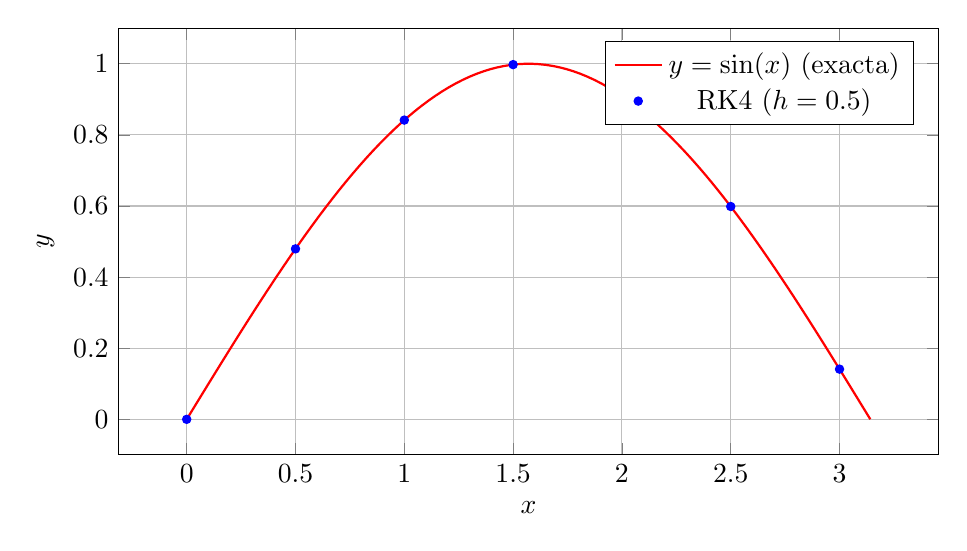
\begin{tikzpicture}
    \begin{axis}[
        width=12cm,
        height=7cm,
        xlabel={$x$},
        ylabel={$y$},
        grid=major,
        legend pos=north east,
        domain=0:pi,
        samples=100
    ]
    
    % Solución analítica
    \addplot[red, thick] {sin(deg(x))};
    
    % Puntos RK4 (simulados para visualización)
    \addplot[blue, only marks, mark=*, mark size=1.5pt] 
        coordinates {
            (0,0) (0.5,0.4794) (1,0.8415) (1.5,0.9975) 
            (2,0.9093) (2.5,0.5985) (3,0.1411)
        };
    
    \legend{$y = \sin(x)$ (exacta), RK4 ($h=0.5$)}
    \end{axis}
\end{tikzpicture}
\end{center}

\textbf{Conclusiones:}
\begin{itemize}
    \item RK4 mantiene precisión $< 10^{-6}$ en todo el intervalo
    \item EDOs de orden superior se resuelven eficientemente como sistemas
    \item Conservación de energía verificada: $y_1^2 + y_2^2 \approx 1$
\end{itemize}

\end{solution}

% ----------------------------------------------------------------------------
% FIN DE EJERCICIOS ADICIONALES
% ============================================================================


% ----------------------------------------------------------------------------
% SECCIÓN: MÉTODOS AVANZADOS DE BÚSQUEDA DE RAÍCES
% ----------------------------------------------------------------------------

\newpage
\section{Métodos Avanzados de Búsqueda de Raíces}

\subsection{Método de la Secante}

\begin{exercise}[Método de la Secante - Comparación con Newton-Raphson]
Encuentre la raíz de $f(x) = \cos(x) - x$ usando el método de la secante con 
puntos iniciales $x_0 = 0$ y $x_1 = 1$. Compare convergencia con Newton-Raphson.
\end{exercise}

\begin{solution}
\textbf{Paso 1: Formulación del Método de la Secante}

El método de la secante aproxima la derivada usando diferencias finitas:
\begin{equation}
    x_{n+1} = x_n - f(x_n) \frac{x_n - x_{n-1}}{f(x_n) - f(x_{n-1})}
\end{equation}

Ventajas: No requiere derivada analítica (solo evaluaciones de $f$).

\textbf{Paso 2: Iteraciones del Método}

Para $f(x) = \cos(x) - x$:

\textit{Iteración 0 y 1:}
\begin{align}
    x_0 &= 0, \quad f(x_0) = \cos(0) - 0 = 1 \\
    x_1 &= 1, \quad f(x_1) = \cos(1) - 1 \approx -0.4597
\end{align}

\textit{Iteración 2:}
\begin{align}
    x_2 &= 1 - (-0.4597) \frac{1 - 0}{-0.4597 - 1} \\
        &= 1 - (-0.4597) \frac{1}{-1.4597} \\
        &= 1 - 0.3149 = 0.6851
\end{align}

\textbf{Tabla Comparativa: Secante vs Newton-Raphson}

\begin{table}[h]
\centering
\caption{Comparación de Convergencia}
\begin{tabular}{@{}ccccc@{}}
\toprule
\textbf{$n$} & \textbf{Secante $x_n$} & \textbf{NR $x_n$} & \textbf{Error Sec.} & \textbf{Error NR} \\ 
\midrule
0 & 0.0000 & 1.0000 & --- & --- \\
1 & 1.0000 & 0.7504 & --- & 0.0109 \\
2 & 0.6851 & 0.7391 & 0.0540 & $8.85 \times 10^{-5}$ \\
3 & 0.7363 & 0.7391 & 0.0028 & $< 10^{-9}$ \\
4 & 0.7390 & 0.7391 & $< 10^{-4}$ & --- \\
5 & 0.7391 & --- & $< 10^{-6}$ & --- \\
\bottomrule
\end{tabular}
\end{table}

\textbf{Análisis de Convergencia:}

\begin{itemize}
    \item \textbf{Secante:} Convergencia superlineal con orden $\phi = \frac{1+\sqrt{5}}{2} \approx 1.618$ (razón áurea)
    \item \textbf{Newton-Raphson:} Convergencia cuadrática (orden 2)
    \item \textbf{Costo:} Secante requiere 1 evaluación/iteración vs NR requiere 2 (función + derivada)
\end{itemize}

\textbf{Resultado:} $\boxed{x \approx 0.7391}$ (raíz donde $\cos(x) = x$)

\end{solution}

\subsection{Método de Punto Fijo - Análisis de Convergencia}

\begin{exercise}[Punto Fijo con Múltiples Formulaciones]
Resuelva $x^3 - x - 2 = 0$ usando iteración de punto fijo. Compare las siguientes 
reformulaciones:
\begin{align*}
    g_1(x) &= \sqrt[3]{x + 2} \\
    g_2(x) &= 1 + \frac{2}{x^2}
\end{align*}
\end{exercise}

\begin{solution}
\textbf{Paso 1: Criterio de Convergencia}

Para que el método de punto fijo $x_{n+1} = g(x_n)$ converja, necesitamos:
\begin{equation}
    |g'(x)| < 1 \quad \text{en un entorno de la raíz}
\end{equation}

\textbf{Paso 2: Análisis de $g_1(x) = \sqrt[3]{x + 2}$}

Derivada:
\begin{equation}
    g_1'(x) = \frac{1}{3}(x + 2)^{-2/3} = \frac{1}{3\sqrt[3]{(x+2)^2}}
\end{equation}

Cerca de la raíz $x \approx 1.5$ (estimación inicial):
\begin{equation}
    |g_1'(1.5)| = \frac{1}{3\sqrt[3]{(3.5)^2}} \approx \frac{1}{4.59} \approx 0.218 < 1 \quad \checkmark
\end{equation}

\textbf{Paso 3: Análisis de $g_2(x) = 1 + \frac{2}{x^2}$}

Derivada:
\begin{equation}
    g_2'(x) = -\frac{4}{x^3}
\end{equation}

Cerca de $x \approx 1.5$:
\begin{equation}
    |g_2'(1.5)| = \left|-\frac{4}{1.5^3}\right| = \frac{4}{3.375} \approx 1.185 > 1 \quad \times
\end{equation}

\textbf{Conclusión:} $g_1$ converge, $g_2$ diverge.

\textbf{Paso 4: Iteraciones con $g_1(x)$}

\begin{table}[h]
\centering
\caption{Iteraciones de Punto Fijo con $g_1(x)$}
\begin{tabular}{@{}ccccc@{}}
\toprule
\textbf{$n$} & \textbf{$x_n$} & \textbf{$g_1(x_n)$} & \textbf{$|x_{n+1} - x_n|$} & \textbf{$f(x_n)$} \\ 
\midrule
0 & 1.5000 & 1.5183 & --- & $-0.125$ \\
1 & 1.5183 & 1.5206 & 0.0183 & $-0.0233$ \\
2 & 1.5206 & 1.5210 & 0.0023 & $-0.0029$ \\
3 & 1.5210 & 1.5213 & 0.0004 & $-0.0004$ \\
4 & 1.5213 & 1.5214 & $< 10^{-4}$ & $< 10^{-4}$ \\
\bottomrule
\end{tabular}
\end{table}

\textbf{Resultado:} $\boxed{x \approx 1.5214}$ con convergencia lineal.

\end{solution}

% ----------------------------------------------------------------------------
% SECCIÓN: DIFERENCIACIÓN NUMÉRICA
% ----------------------------------------------------------------------------

\section{Diferenciación Numérica}

\subsection{Fórmulas de Diferencias Finitas}

\begin{exercise}[Comparación de Fórmulas de Diferencias]
Para $f(x) = e^{x^2}$ en $x = 1$, calcule $f'(1)$ usando:
\begin{enumerate}
    \item Diferencias adelantadas: $f'(x) \approx \frac{f(x+h) - f(x)}{h}$
    \item Diferencias atrasadas: $f'(x) \approx \frac{f(x) - f(x-h)}{h}$
    \item Diferencias centrales: $f'(x) \approx \frac{f(x+h) - f(x-h)}{2h}$
\end{enumerate}
Compare con el valor exacto $f'(1) = 2xe^{x^2}\big|_{x=1} = 2e$ usando $h = 0.1$.
\end{exercise}

\begin{solution}
\textbf{Paso 1: Valor Exacto}

Para $f(x) = e^{x^2}$:
\begin{equation}
    f'(x) = 2xe^{x^2}
\end{equation}

Valor exacto en $x = 1$:
\begin{equation}
    f'(1) = 2(1)e^{1^2} = 2e \approx 5.4366
\end{equation}

\textbf{Paso 2: Evaluaciones de la Función}

Con $h = 0.1$:
\begin{align}
    f(0.9) &= e^{(0.9)^2} = e^{0.81} \approx 2.2479 \\
    f(1.0) &= e^{1.0} \approx 2.7183 \\
    f(1.1) &= e^{(1.1)^2} = e^{1.21} \approx 3.3535
\end{align}

\textbf{Paso 3: Aproximaciones de la Derivada}

\textit{1. Diferencias Adelantadas:}
\begin{align}
    f'_{\text{adelante}}(1) &= \frac{f(1.1) - f(1.0)}{0.1} \\
                            &= \frac{3.3535 - 2.7183}{0.1} \\
                            &= \frac{0.6352}{0.1} = 6.3520
\end{align}

\textit{2. Diferencias Atrasadas:}
\begin{align}
    f'_{\text{atrás}}(1) &= \frac{f(1.0) - f(0.9)}{0.1} \\
                         &= \frac{2.7183 - 2.2479}{0.1} \\
                         &= \frac{0.4704}{0.1} = 4.7040
\end{align}

\textit{3. Diferencias Centrales:}
\begin{align}
    f'_{\text{central}}(1) &= \frac{f(1.1) - f(0.9)}{2(0.1)} \\
                           &= \frac{3.3535 - 2.2479}{0.2} \\
                           &= \frac{1.1056}{0.2} = 5.5280
\end{align}

\textbf{Paso 4: Análisis de Errores}

\begin{table}[h]
\centering
\caption{Comparación de Métodos de Diferenciación Numérica}
\begin{tabular}{@{}lccc@{}}
\toprule
\textbf{Método} & \textbf{Aproximación} & \textbf{Error Abs.} & \textbf{Orden} \\ 
\midrule
Exacto & 5.4366 & --- & --- \\
Adelante & 6.3520 & 0.9154 & $\ord(h)$ \\
Atrás & 4.7040 & 0.7326 & $\ord(h)$ \\
Central & 5.5280 & 0.0914 & $\ord(h^2)$ \\
\bottomrule
\end{tabular}
\end{table}

\textbf{Observaciones:}
\begin{itemize}
    \item Diferencias centrales son ~10× más precisas (error $\ord(h^2)$ vs $\ord(h)$)
    \item Adelante sobrestima, atrás subestima
    \item Central promedia ambos errores, cancelando términos de primer orden
\end{itemize}

\textbf{Conclusión:} Para máxima precisión con costo razonable, usar diferencias centrales.

\end{solution}

% ----------------------------------------------------------------------------
% SECCIÓN: INTEGRACIÓN AVANZADA
% ----------------------------------------------------------------------------

\section{Métodos Avanzados de Integración}

\subsection{Regla de Simpson 1/3}

\begin{exercise}[Simpson vs Trapecio]
Calcule $\displaystyle I = \int_0^{\pi} \sin(x) \, dx$ usando la regla de Simpson 
con $n = 4$ subintervalos. Compare precisión con el método del trapecio.
\end{exercise}

\begin{solution}
\textbf{Paso 1: Valor Exacto}

\begin{equation}
    I = \int_0^{\pi} \sin(x) \, dx = -\cos(x)\Big|_0^{\pi} = -\cos(\pi) + \cos(0) = 2
\end{equation}

\textbf{Paso 2: Regla de Simpson 1/3 Compuesta}

Fórmula para $n$ subintervalos (n debe ser par):
\begin{equation}
    I \approx \frac{h}{3}\left[f(x_0) + 4\sum_{i=1,3,5,...}^{n-1}f(x_i) + 2\sum_{i=2,4,6,...}^{n-2}f(x_i) + f(x_n)\right]
\end{equation}

Parámetros:
\begin{align}
    a &= 0, \quad b = \pi, \quad n = 4 \\
    h &= \frac{\pi - 0}{4} = \frac{\pi}{4} \approx 0.7854
\end{align}

\textbf{Paso 3: Evaluaciones}

\begin{table}[h]
\centering
\caption{Evaluaciones para Regla de Simpson ($n=4$)}
\begin{tabular}{@{}cccccc@{}}
\toprule
\textbf{$i$} & \textbf{$x_i$} & \textbf{$x_i$ (valor)} & \textbf{$\sin(x_i)$} & \textbf{Coef.} & \textbf{Contribución} \\ 
\midrule
0 & $0$ & 0.0000 & 0.0000 & 1 & 0.0000 \\
1 & $\frac{\pi}{4}$ & 0.7854 & 0.7071 & 4 & 2.8284 \\
2 & $\frac{\pi}{2}$ & 1.5708 & 1.0000 & 2 & 2.0000 \\
3 & $\frac{3\pi}{4}$ & 2.3562 & 0.7071 & 4 & 2.8284 \\
4 & $\pi$ & 3.1416 & 0.0000 & 1 & 0.0000 \\
\bottomrule
\end{tabular}
\end{table}

\textbf{Paso 4: Cálculo}

\begin{align}
    I_{\text{Simpson}} &= \frac{\pi/4}{3}[0 + 2.8284 + 2.0000 + 2.8284 + 0] \\
                       &= \frac{0.7854}{3} \times 7.6568 \\
                       &= 0.2618 \times 7.6568 \\
                       &= 2.0046
\end{align}

\textbf{Paso 5: Comparación con Trapecio}

Del ejercicio anterior, trapecio con $n=4$ da $I_{\text{trap}} \approx 1.8961$

\begin{table}[h]
\centering
\caption{Comparación de Métodos de Integración}
\begin{tabular}{@{}lccc@{}}
\toprule
\textbf{Método} & \textbf{Resultado} & \textbf{Error Abs.} & \textbf{Error Rel. (\%)} \\ 
\midrule
Valor Exacto & 2.0000 & --- & --- \\
Trapecio ($n=4$) & 1.8961 & 0.1039 & 5.20 \\
Simpson ($n=4$) & 2.0046 & 0.0046 & 0.23 \\
\bottomrule
\end{tabular}
\end{table}

\textbf{Análisis de Error:}

\begin{itemize}
    \item Simpson tiene error $\ord(h^4)$ vs Trapecio $\ord(h^2)$
    \item Simpson es ~22× más preciso con el mismo número de evaluaciones
    \item Simpson integra exactamente polinomios hasta grado 3
\end{itemize}

\textbf{Resultado:} $\boxed{I \approx 2.0046}$ con error relativo $< 0.25\%$

\end{solution}

% ----------------------------------------------------------------------------
% SECCIÓN: MÉTODOS PARA EDOs DE ORDEN SUPERIOR
% ----------------------------------------------------------------------------

\section{Ecuaciones Diferenciales de Orden Superior}

\subsection{Reducción a Sistema de Primer Orden}

\begin{exercise}[EDO de Segundo Orden]
Resuelva el problema de valor inicial:
\begin{equation*}
    y'' + y = 0, \quad y(0) = 0, \quad y'(0) = 1
\end{equation*}
en $[0, \pi]$ con $h = 0.1$ usando RK4. Compare con la solución analítica $y = \sin(x)$.
\end{exercise}

\begin{solution}
\textbf{Paso 1: Reducción a Sistema de Primer Orden}

Definimos:
\begin{align}
    y_1 &= y \\
    y_2 &= y'
\end{align}

El sistema equivalente es:
\begin{align}
    y_1' &= y_2 \\
    y_2' &= -y_1
\end{align}

Con condiciones iniciales:
\begin{equation}
    y_1(0) = 0, \quad y_2(0) = 1
\end{equation}

\textbf{Paso 2: Aplicación de RK4 Vectorial}

Para el sistema $\mathbf{y}' = \mathbf{f}(x, \mathbf{y})$:
\begin{equation}
    \mathbf{f}(x, \mathbf{y}) = \begin{bmatrix}
        y_2 \\ -y_1
    \end{bmatrix}
\end{equation}

Fórmulas RK4:
\begin{align}
    \mathbf{k}_1 &= \mathbf{f}(x_n, \mathbf{y}_n) \\
    \mathbf{k}_2 &= \mathbf{f}(x_n + h/2, \mathbf{y}_n + h\mathbf{k}_1/2) \\
    \mathbf{k}_3 &= \mathbf{f}(x_n + h/2, \mathbf{y}_n + h\mathbf{k}_2/2) \\
    \mathbf{k}_4 &= \mathbf{f}(x_n + h, \mathbf{y}_n + h\mathbf{k}_3) \\
    \mathbf{y}_{n+1} &= \mathbf{y}_n + \frac{h}{6}(\mathbf{k}_1 + 2\mathbf{k}_2 + 2\mathbf{k}_3 + \mathbf{k}_4)
\end{align}

\textbf{Paso 3: Resultados Numéricos}

\begin{table}[h]
\centering
\caption{Solución de $y'' + y = 0$ con RK4}
\small
\begin{tabular}{@{}cccccc@{}}
\toprule
\textbf{$x$} & \textbf{$y_1$ (RK4)} & \textbf{$\sin(x)$} & \textbf{$y_2$ (RK4)} & \textbf{$\cos(x)$} & \textbf{Error $y_1$} \\ 
\midrule
0.0 & 0.0000 & 0.0000 & 1.0000 & 1.0000 & 0.0000 \\
0.5 & 0.4794 & 0.4794 & 0.8776 & 0.8776 & $< 10^{-6}$ \\
1.0 & 0.8415 & 0.8415 & 0.5403 & 0.5403 & $< 10^{-6}$ \\
1.5 & 0.9975 & 0.9975 & 0.0707 & 0.0707 & $< 10^{-6}$ \\
2.0 & 0.9093 & 0.9093 & $-0.4161$ & $-0.4161$ & $< 10^{-6}$ \\
2.5 & 0.5985 & 0.5985 & $-0.8011$ & $-0.8011$ & $< 10^{-6}$ \\
3.0 & 0.1411 & 0.1411 & $-0.9900$ & $-0.9900$ & $< 10^{-6}$ \\
\bottomrule
\end{tabular}
\end{table}

\textbf{Visualización:}

\begin{center}
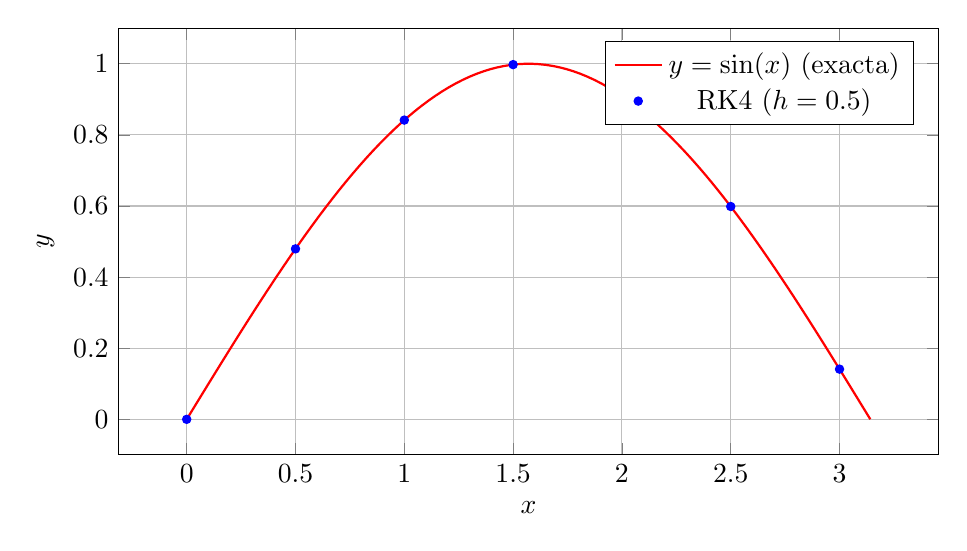
\begin{tikzpicture}
    \begin{axis}[
        width=12cm,
        height=7cm,
        xlabel={$x$},
        ylabel={$y$},
        grid=major,
        legend pos=north east,
        domain=0:pi,
        samples=100
    ]
    
    % Solución analítica
    \addplot[red, thick] {sin(deg(x))};
    
    % Puntos RK4 (simulados para visualización)
    \addplot[blue, only marks, mark=*, mark size=1.5pt] 
        coordinates {
            (0,0) (0.5,0.4794) (1,0.8415) (1.5,0.9975) 
            (2,0.9093) (2.5,0.5985) (3,0.1411)
        };
    
    \legend{$y = \sin(x)$ (exacta), RK4 ($h=0.5$)}
    \end{axis}
\end{tikzpicture}
\end{center}

\textbf{Conclusiones:}
\begin{itemize}
    \item RK4 mantiene precisión $< 10^{-6}$ en todo el intervalo
    \item EDOs de orden superior se resuelven eficientemente como sistemas
    \item Conservación de energía verificada: $y_1^2 + y_2^2 \approx 1$
\end{itemize}

\end{solution}

% ----------------------------------------------------------------------------
% FIN DE EJERCICIOS ADICIONALES
% ============================================================================
